\section{Metaheur\'istica GRASP}

La metaheur\'istica GRASP utiliza los dos algoritmos anteriormente explicados combinados de tal manera de combinar lo mejor de ambos mundos.

Las deficiencias, en t\'erminos generales, que tiene la b\'usqueda local es que depende mucho de la semilla o la soluci\'on general.

\begin{figure}[H]
        \centering
        \begin{subfigure}[b]{0.7\textwidth}
                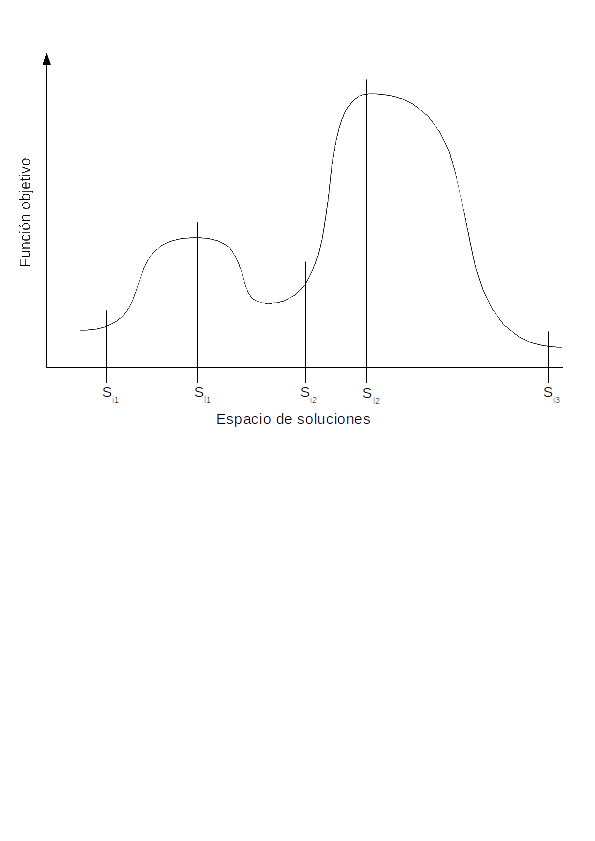
\includegraphics[width=\textwidth]{ej5/local1.png}
                \caption{Problemas con la busqueda local}
                \label{fig:prob_con_bl}
        \end{subfigure}%
\end{figure}

en la figura de arriba podemos apreciar que de empezar por $s_{i1}$ se llegar\'ia a una soluci\'on $s_{l1}$, pero nunca a la $s_{l2}$ que es la mejor de las dos.

Para evitar esto se puede empezar por alguna soluci\'on random, pero esto tiene el problema que es poco probable que la soluci\'on sea buena. Por ejemplo $s_{i3}$ est\'a m\'as lejos en el espacio de soluciones y en cuan \'optima es seg\'un la funci\'on objetivo, lo cual llevar\'ia a que la b\'usqueda local deba hacer muchas iteraciones hasta encontrar $S_{l2}$.

Se puede usar un algoritmo golozo que son mejores que una soluci\'on random, con alg\'un tipo de randomizaci\'on para evitar que siempre arrojen la misma soluci\'on.

\subsection{Algoritmo}



\subsection{Experimentaci\'on}
